\documentclass[11pt]{article}
\usepackage[greek,english]{babel}
\usepackage{apacite}
\usepackage{natbib}
\usepackage[utf8]{inputenc}
\usepackage{amsmath}
\usepackage{graphicx}
\graphicspath{{images/}}
\usepackage{fancyhdr}
\usepackage{multicol}
\usepackage{vmargin}
\usepackage{lscape}
\usepackage[table,xcdraw]{xcolor}
\usepackage{parskip}
\usepackage{longtable}
\usepackage{caption}
%\usepackage{subcaption}
\usepackage[nottoc]{tocbibind}
\usepackage{siunitx}
\usepackage{commath}
\usepackage{listings}
\usepackage{color}
\usepackage{amsmath}
\usepackage{textgreek}
\usepackage{hyperref}
\usepackage{subfig}
\setmarginsrb{20mm}{20mm}{20mm}{20mm}{10pt}{10mm}{10pt}{10mm}



\begin{document}
% Create a title page for your document
\begin{titlepage}
    \begin{center}

			{\huge\bfseries Magneto-hydrodynamics in Population III star formation\par}
			\vspace{2cm}
			{\Large\itshape Lewis Prole\par}
			\vfill
			supervised by\par
			Paul Clark

			\vfill


    \end{center}
\end{titlepage}

% Creates table of contents
\tableofcontents
\thispagestyle{empty}

\newpage
\setcounter{page}{1} % Starts the page numbering (at 1) after all contents pages
\section{Introduction} % (fold)
\label{sec:intro}

\subsection{Primordial conditions and structure formation}
\label{sub:prim_cond}

Initially, the Universe was too hot and dense for ions and electrons to combine, matter existed as an ionised plasma. The temperature of the universe dropped for $\sim\num{3.7e5}$yrs before it was cool enough for atoms to form, this is known as recombination and occurred at a redshift of $\sim1100$. The primordial plasma was efficient at scattering radiation, so it is impossible to observe events before recombination. However, the neutral atoms resulting from recombination could not interact with radiation, allowing it to freely stream, forming the cosmic microwave background (CMB). From CMB calculations, \citet{Peebles1966} showed that a large amount of 4He, along with smaller amounts of lighter elements were produced in the big bang, giving a primordial He abundance of $\sim25\%$. It is now known that the abundances relative to hydrogen were $\sim\num{1e-5}$ for D and 3He and $\sim\num{1e-7}$ for 7Li \citep{Copi1995}. In these \emph{Cosmic Dark Ages}, the Universe remained neutral until the formation of the first (Population III) stars, whos UV radiation heated and ionised the ISM around them \citep{Bromm2001} at the epoch of \emph{Reionisation}. The ISM was enriched  with heavy elements for the first time when these Population III (Pop III) stars died as supernovae \citep{Heger2003}.
In a cold dark matter ($\Lambda$CDM) Universe, the formation of these Population III (Pop III) stars began with hierarchical structure formation, starting with the formation of low mass, dark matter (DM) haloes \citep{Couchman1986}.
In order for baryonic gas to collapse within these haloes, it needed to cool. As layed out in \cite{Bromm2002}, H$_{2}$ was the main coolant in DM halos, due to the absence of dust grains and heavy elements. At temperatures expected in collapsing Pop III objects ($<$\num{e4}K), rotational transitions can only occur via electrical quadrupole radiation with small transition probabilities because H$_{2}$ possesses no determinant dipole moment. The formation of H$_{2}$ primarily occurs via the H$^{-}$ channel

\begin{equation}
\begin{split}
H + e^{-} \rightarrow H^{-} + h\nu
\\
H^{-} + H \rightarrow H_{2} + e^{-}
\end{split}
\end{equation}

for redshifts z$<$100, where the CMB cannot destroy  H$^{-}$. As there is no way to ionise H at such low temperatures, the residual abundance of free electrons from the big bang is used for the reaction. The resultant abundance of H$_{2}$ was calculated as  $\sim$ \num{e-4}-\num{e-3}. The maximum cooling rate of H$_{2}$ is set by the transition from not local thermal equilibrium (LTE) to LTE, at the critical density of $\sim$ \num{e3}-\num{e4}cm$^{-3}$. The minimum temperature attainable due to H$_{2}$ cooling is then 500K, but the Maxwellian velocity distribution tail allows real minimum temperatures of $\sim$100K. This allowed gas to collapse into high density structures of $n >$ \num{e8}cm$^{-3}$. Another possible coolant is HD, which becomes significant in the later stages of collapse ($\sim$ 100-300K) despite its low abundance (\num{e-5}$n_{H}$), due to its permanent electric dipole and relatively larger transitional probabilities. 
Simulations of early structure formation in a $\Lambda$CDM Universe indeed show the formation of these dark matter minohalos. \cite{Yoshida2003} found halos of mass $\sim\num{1e6}$ M\textsubscript{\(\odot\)} collapsing at redshifts z$\sim$20–30. Within these haloes, the virial temperatures were too low ($\sim$2000K) for cooling via atomic hydrogen lines ($>\num{1e4}$K), but efficient rotational line cooling by molecular hydrogen allowed formation of cold dense gas clumps. The DM and baryonic matter have relative velocities with respect to one another, owing to residual velocity fluctuations in the baryonic component, dating from the epoch when the baryons and photons were strongly coupled  \citep{Tseliakhovich2010}. \cite{Schauer2019} showed that increasing the streaming velocity makes it harder for baryonic matter to settle into DM haloes, decreases the number of halos formed due to lower self-gravity in over-dense regions, and increasing the minimum halo mass. They also found that increased streaming velocities increases the minimum halo mass needed for efficient H2 cooling, and hence Pop III star formation. They found that for $v>3v$\textsubscript{rms}, H2 cooling was completely suppressed, so that star formation could only occur in ‘atomic cooling haloes’.



\subsection{Primordial stars}
\label{sub:presVSprim}
Polytropic relations between pressure and density $P \propto \rho^\gamma$ are commonly used to describe the thermal evolution of gas during cloud collapse (e.g. \citealt{Hennebelle2008}, \citealt{Machida2008a}, \citealt{Tomisaka2002}). In present day star formation, gas initially collapses isothermally ($\gamma \sim 1$) up until the central density $n$ reaches $\sim$ \num{e11}cm$^{-3}$, where the gas becomes adiabatic ($\gamma \sim 5/3$) and the 'first core' is formed. Molecular hydrogen is dissociated at  $n \sim$ \num{e16}cm$^{-3}$ and the polytropic index becomes $\gamma \sim$ 1.1 allowing rapid collapse. A protostar forms at at $n \sim$ \num{e21}cm$^{-3}$ where the equation of state becomes stiff ($\gamma \sim 5/3$). The lack of metal coolants and dust grains in primordial gas clouds changes the thermal evolution from the present day scenario. Calculations show that primordial clouds were at $\sim$200K at \num{e11}cm$^{-3}$, with $\gamma \sim 1.1$ at these lower densities, owing to H$_{2}$ cooling (e.g. \citealt{Omukai1998}). As described in \cite{McKee2008}, collapse after the formation of dense H$_{2}$ clumps is subject to feedback effects. As the protostar accretes, it emits nonionising UV radiation capable of photodissociating H$_{2}$ , raising the adiabatic index $\gamma$ from 1.1 to 5/3. The raise in adiabatic index does not prevent further accretion in clumps that have already formed a protostar, but can prevent further collapse in nearby clumps that are yet to form a protostar, so the UV feedback can suppress star formation in the vicinity of a protostar. Extreme UV radiation from the protostar can ionise infalling neutral gas, creating a H\textsubscript{II} region around the protostar, the increased temperature gives the ionised gas higher pressure than the surrounding neutral gas, despite being the same density. The pressure gradient allows the H\textsubscript{II} region to expand, reducing accretion. Ly$\alpha$ photons from the H\textsubscript{II} region are trapped by the high column density of neutral gas outside the H\textsubscript{II}  region, amplifying the radiation pressure until Ly$\alpha$ photons can escape from the poles, reducing the radiation pressure. \cite{Omukai2005} showed that the thermal evolution of star forming clouds with different metallicities converge at $\sim$\num{e16}cm$^{-3}$, or \num{4e-8}gcm${-3}$ for primordial clouds (\autoref{fig:thermal}). For densities above \num{1e16}cm$^{-3}$, gas collapse is the same for both present day and primordial clouds. 

With observations of high redshift ($z \sim$ 10) sources in the Near Infrared Camera and Multi-Object Spectrometer (NICMOS) Hubble Ultra Deep Field (HUDF), \cite{Choudhury2006} found that Pop III stars began hydrogen reionization at $z \sim$ 15, and that reionisation was 90 per cent complete by $z \sim$ 10, assuming a Salpeter initial mass function (IMF). In a large-volume, high-resolution simulations of cosmic reionization, \citet{Trac2007} found that the complete overlap of ionised H\textsubscript{II} regions occurred at $z \sim$ 6.5, assuming a top-heavy IMF. It is theorised that low mass Pop III stars that were ejected from their DM halo could still be active today, \cite{Hartwig2015} calculated the number of expected  Pop III survivors assuming a logarithmically flat IMF, and estimated the probability of detecting them. \cite{Magg2019} ruled out those predictions along with those of \cite{Ishiyama2016}, by calculating the probability of the non-detection  of Pop III survivors up until now, concluding that low mass Pop III stars must have formed more rarely than currently thought, or that they are polluted by metals during their lifetime. Pollution in this way was investigated by \cite{Frebel2009}, who found that interstellar accretion had a negligible effect on the surface abundances of metal-poor stars, while \cite{Johnson2011} found that a solar-like wind produced by the Pop III stars would be essential to prevent significant accretion, although the existence of such winds is unknown. At the end of their lives, high mass Pop III stars explode as supernova (SN), enriching the ISM with metals e.g., O, Mg, Si, and Fe (e.g. \citealt{Tominaga2007}). \cite{Iwamoto2005} argued that observed hyper-metal-poor stars originally presented as possible Pop III observations, are actually second generation stars (Pop II), formed in gas clouds enriched by Pop III SN. \cite{Smith2018} showed that black holes from Pop III remnants do not display efficient mass accretion and are not the initial seeds for a significant population of intermediate black holes in the early universe. They found that star formation competes with black hole growth through gas accretion and feedback. 

The assumed IMF effects reionisation calculations, predictions about surviving low-mass Pop III stars, and SN enrichment estimates, yet the above studies are not consistent with their choice of IMF, and there is still no consensus on which IMF is most appropriate. Investigations on the Pop III IMF are ongoing (e.g. \citealt{Ma2017a}).

\begin{figure*}[h!]
         \centering
		\includegraphics[width=17cm]{thermal.png}
		\caption{Thermal evolution of gas in star forming clouds with different metallicities $Z$, where the diagonal dashed lines are lines of constant Jeans mass. [Z/H]=-$\infty$ corresponds to 0 metallicity i.e a primordial gas cloud. \citep{Omukai2005} }
		\label{fig:thermal}
\end{figure*}





\subsection{A primordial magnetic field}
\label{sub:Bfield}
Astrophysicists have investigated primordial magnetic fields to explain the origin of present day galactic magnetic fields. Magnetic dynamos \citep{Vainshtein1980} have been invoked to convert kinetic energy of the electrically conductive medium into magnetic energy. In this scenario, a non-vanishing seed field would be needed to initiate the dynamo, along with turbulence and global rotation, to amplify the field. On the other hand, primordial fields have been suggested (e.g. \citealt{Kulsrud1990}), whereby the magnetic field is amplified due to the conservation of magnetic flux during the collapse of a protogalactic cloud. In both scenarios, an initial field is required to explain the galactic field. A strong primordial magnetic field would have also impacted big bang nucleosynthesis (BBN), increasing the $\beta$ decay rate of neurons \citep{Matese1969}, lowering the relic abundance of He from BBN.  \cite{Greenstein1969} argued that a primordial field did not exist, as it would result in too much helium or too much deuterium and helium-3. The relic abundance of He has been used to put constraints on the magnetic field strength at nucleosynthesis time. \cite{Grasso1996} found that the main effects of primordial magnetic fields on BBN are its effect on the Universe expansion rate from its contribution to the energy density, and the fields effect on quantum statistics. They found an upper limit on field strength as B$<$\num{1e11}G for a homogeneous field at T=1\num{1e9}K. When the field was generalised to inhomogeneous on horizon scales, the limit increased to \num{1e12}G.
\cite{Barrow1997} used data from the 4-year Cosmic Background Explorer (COBE), to calculate the effects of a general homogenous gravitational field on the temperature anisotropy of the CMBR. They used this to give an upper limit on the primordial field at recombination of B\textsubscript{0}=\num{3.4e-9}($\Omega$\textsubscript{0}h\textsubscript{50}\textsuperscript{2})\textsuperscript{1/2}G.
\cite{Silk2006}  argued that even when starting in an unmagnetized medium, radiation drag or thermal pressure could generate magnetic field seeds in the discs surrounding the first protostellar objects. As the central object grows through accretion, the rotational velocity increases, acting to reducing the minimum field strength needed for magnetio-rotational instability (MRI). Once the minimum value falls lower than the field generated in the disc, the resulting MRI dynamo would enhance the field strength and drive ejections from the protostar.







\subsection{MHD $\&$ jets}
\label{sub:MHD}
In the limit of a zero resistivity plasma (ideal MHD limit) with a magnetic Reynolds number $\Re_{M}>1$, \cite{Alfven1942} showed that magnetic fields deform with the movement of a plasma, a phenomenon known as \emph{flux-freezing}. As a consequence of flux-freezing, if a column of plasma is bent, twisted or distorted, the magnetic field lines through the column will bend, twist or distort with it. Two points connected by a field line will remain connected by the field line, so when a cloud of gas collapses, the magnetic flux through the cloud remains constant, amplifying the magnetic field as the surface area decreases. Upon perturbing an ideal MHD plasma, the disturbance propagates as two waves. The first is called the \emph{Alfven wave}, where the disturbance acts transverse to the wave direction, and moves paralel to the field line as a non compressive wave at the \emph{Alfven speed}, driven by magnetic tension attempting to oppose the displacement. The second wave is split into \emph{fast} and \emph{slow magnetoaccoustic waves}. These waves are longitudinal and compressive, with the fast wave propergating perpendicular to the field lines, while the slow wave propergates parallel to the field. From \emph{Ferraro's law of isorotation} \citep{Ferraro1937}, a rotating cloud with symmetry around the axis of ration in a uniform poloidal magnetic field, can only be in a steady state if angular velocity is constant along the magnetic field lines. When the angular velocity is lower outside of the cloud, the field lines are distorted, creating toroidal field lines from the initially poloidal field. Magnetic tension acts to correct the distortion by transferring angular momentum to the slower regions, which is known as \emph{magnetic breaking}. In solar winds, the angular velocity decreases with distance from the sun. The magnetic tension transports angular momentum through the wind, establishing a near-rigid rotation. This works up to the \emph{Alfven radius}, where the magnetic energy drops below the rotational energy of the wind, at which point the angular velocity becomes lower than that at the solar surface and the magnetic field lines become twisted. \cite{Blandford1982} developed a hydromagnetic jet model in which centrafugal forces drive the plasma out of the accretion disk and along magnetic field lines if they make an angle with the disk $<60deg$. In this model, field lines are initially poloidal and frozen into the disk, the inertia of the gas above the disk bends the field lines into an increasingly toroidal field. The magnetic stress associated with the twisting forces then causes the outflow to become collimated, where the final shape of the magnetic structure is determined by an equilibrium between in the inward magnetic hoop stress and the outward magnetic pressure. \cite{Lynden-Bell1996} explained that this 'pinching' effect is caused by the concentration of an external pressure by the toroidal field. Their model was split into three sections; close to the disk where magnetic pressure $B^{2}/8\pi$ exceeds external pressure $p$, where the field grows outwardly within a cone of $\sim 60\deg$. This was followed by a cylindrical section II, where a force-free magnetic structure of twisted field lines  grows in height with successive turns of the disk, surrounded by a sheet where $B^{2}/8\pi$  is balanced by $p$. Finally, at the top of the structure, the upwards pressure of the field is balanced by the ambient pressure and the field lines bend over to return downwards through section II, at a greater cylindrical radius than the upward flux. \cite{Lynden-Bell2003}  showed in the presence of an external pressure surrounding a force-free magnetic field, the toroidal field lines give a potential energy minimum condition satisfied if the height of the magnetic tower increases linearly with successive disk turns. 

\subsection{Hydrodynamic codes}
\subsubsection{Numerical effects}
\label{sub:numerical}
When simulating the physical world with hydrostatic codes, finite errors are unavoidable and deviate the evolution from the initial conditions to the final result. These errors are not limited to the underlying physics of the code, numerical effects can also lead to non-physical results. Perturbations with scale length larger than the Jeans length $\lambda_{J}$ are unable to support themselves via thermal pressure against self-gravity. During an isothermal collapse, the Jeans length decreases. The \emph{Jeans requirement} requires that $\lambda_{J}$ must not fall below the resolution (cell size $\Delta x$) of a simulation. Failure to satisfy this condition results in artificial instability and collapse. Furthermore, the \emph{Truelove condition} \citep{Truelove1997} states that in order to prevent finite numerical errors correlated on scales $>\lambda_{J}$ from condensing into artificial fragmentations, the Jeans number $\Delta x/\lambda_{J}$ must be at least as low as 0.25, corresponding to at least 4 cells per Jeans length. Another condition for stability is known as the Courant, Friedrichs and Lewy (CFL) limitation \citep{Courant1952}, which states that information must not be allowed to travel further than the cell length during a timestep, such that information from a cell can only be communicated to its immediate neighbours. The \emph{Courant number} is defined as the ratio \citep[p.~70]{LeVeque2002}

\begin{equation}
\nu \equiv \abs{\frac{\hat{u}\Delta t}{ \Delta x} }
\end{equation}

 where $\Delta t$, $\Delta x$ and $\hat{u}$ are the  the time step, the cell size and the characteristic wave speed of the system, respectively.
 
Maxwell's equations state that 
 
 \begin{equation}
\nabla \cdot B = 0\label{eq:divb}
\end{equation}

In other words, magnetic fields have zero divergence. However, simulation codes generate divergent fields from initially non-divergent fields, which clearly must be cleaned to prevent non-physical results. The divergence cleaning is handled differently for grid codes (e.g. \citealt{Jiang2012}) and smoothed particle codes (e.g. \citealt{Ziegler2006}).

\subsubsection{Finite volume solver}
\label{sub:finite}
Failure to conserve conserved quantities like density and momentum also leads to non-physical results. For a given cell, finite volume solvers evolve conserved quantities in time based on the flux of those quantities, at the boundaries to the cells around them. For a conserved quantity $q_{x}^{t}$ at position $x$ and time $t$, the fluxes $f_{x}^{t}$ are calculated at the boundaries $f_{i-1/2}$ and $f_{i+1/2}$, evaluated at a half-time step $f^{n+1/2}$, the flux-conserving advection equation becomes 

 \begin{equation}
q_{i}^{n+1}=q_{i}^{n} + \frac{\Delta t}{\Delta{x}}(f_{i-1/2}^{n+1/2}-f_{i+1/2}^{n+1/2}) \label{eq:advect}
\end{equation}

where 

\begin{equation}
 f_{i+1/2}^{n+1/2}= q_{i+1/2}^{n+1/2}u_{i+1/2}\label{eq:advect2}
\end{equation}

and $u_{i+1/2}$ is the advection velocity at the boundary. This requires an estimate of $q$ at the boundary. The Donor-cell advection scheme assumes that $q$ is constant across the cells, and the cell boundary adopts either $q_{n}$ if $u_{n+1/2}$ is positive or $q_{n+1/2}$ if $u_{n+1/2}$ is negative. On the other hand, the Piecewise linear scheme assumes that $q$ is a linear function from the center of a cell to the next. A sub-grid is created and the distribution of $q$ is reconstructed with the new linear variation within the original cells.


\subsection{AREPO}
\label{sub:arepo}
Arepo improves upon the failures of previous hydrodynamic simulation techniques, namely adaptive mesh refinement and smoothed particle hydrodynamics. The Eulerian approach to fluid dynamics involves a cartesian mesh where fluid properties flow through control volumes, adaptive mesh refinement (AMR: \citealt{Berger1989}) allows patches of finer mesh spacing to be placed in areas suffering from high errors. An advantage of this approach is that entropy is implicitly produced when fluxes of different thermodynamic states are mixed in a cell. \cite{Wadsley2008} showed that numerical diffusion attributable to advection terms in Eulerian methods are sensitive to bulk motions of the fluid relative to the mesh, giving a lack of Galilean invariance. They also displayed that AMR may be subject to overmixing due to numerical viscosity and non-Galilean invariant diffusion, causing inaccuracies in entropy tracking. \cite{Heitmann2008} demonstrated that AMR codes struggle with gravitational instability driven structure formation, as refinement was discontinuous and couldn’t keep up with small density fluctuations. In contrast, the Lagrangian approach is to follow individual fluid elements as they move around an enclosing volume. Smoothed particle hydrodynamics (SPH: \citealt{Monaghan1992}) follows this approach, calculating gas properties of individual particles by averaging over its nearest neighbours. Unlike AMR, SPH does not have implicit entropy production through mixing. \cite{Moore2000} displayed that SPH suffers inaccuracies due to poor shock capturing resolution compared to AMR. \cite{Agertz2007} demonstrated that SPH codes poorly handle situations with steep density gradients, causing erroneous pressure forces and decoupling different phases of the fluid. AREPO displays both Euerian and Lagrangian properties, in that it is a mesh code, but that the mesh is a moving, unstructured, Voronoi tessellation of discrete points (see \autoref{fig:voroni}). AREPO solves hyperbolic conservation laws of ideal hydrodynamics with a finite volume approach, based on a second-order unsplit Godunov scheme with an exact Riemann solver \citep{Springel2010}. Automatic and continuous refinement overcome the challenge of structure growth associated with AMR, yet the Eularian properties overcome poor shock capturing resolution associated with SPH, while remaining Galilean-invariant. 

\begin{figure*}[h!]
         \centering
		\includegraphics[width=8cm]{Voroni.png}
		\caption{Voroni tessellation in 2D for a set of random cell positions (red dots) \citep{Springel2010}}
		\label{fig:voroni}
\end{figure*}

\subsubsection{Radiative feedback for Primordial chemistry}
SPRAI (Simplex Photon Radiation in the Arepo Implementation: \citealt{Jaura2018}) is a radiative transfer (RT) code for primordial chemistry, based on the SIMPLEX radiation transfer method, implimented with AREPO. SIMPLEX (\citealt{Ritzerveld2006}, \citealt{Kruip2010}) is a method where photons are transported on an unstructured Delaunay triangulation, Unlike Monte Carlo or ray tracing methods, the computational cost of the SIMPLEX method does not scale directly with the number of sources. SIMPLEX has previously been used only in post processing, while SPRAI is directly integrated into the AREPO code, for 'on-the-fly' use. Sources inject new photons into cells, which are transferred from cell to cell in a sequence of RT steps. The movement of photons allows calculation of fluxes and ionization rates in each cell. SPRAI uses an integrated chemistry model that includes ionization, recombination, and cooling of hydrogen and helium in several frequency bins. Photons are propagated until they are completely attenuated in the gas, and travel with infinite speed. For this reason, SPRAI may not be suitable for large cosmological simulations where the box size exceeds $ct$ where $t$ is the time step, and $c$ is the speed of light.

\subsubsection{MHD divergence cleaning}
Numerically generated divergence in magnetic fields yield unphysical results and instability, the \cite{Dedner2002} hyperbolic divergence cleaning scheme invokes an unknown function $\psi$ to couple the divergence condition (\ref{eq:divb}) to the ideal MHD equations. This allows for a mixed hyperbolic/parabolic correction to be added to the MHD equation, which dissipates and propagates divergence errors to the boundary with finite speed. Density, momentum, magnetic induction, and total energy density are conserved during the correction. The correction is easily added to the existing MHD modules in AREPO by introducing a generalized Lagrange multiplier.



\subsection{Simulations of star formation}
\subsubsection{MHD in present-day star formation}
\label{sub:MHD_present}

There are a wealth of studies on present day star formation in the presence of magnetic fields. \cite{Machida2005} used three-dimensional magnetohydrodynamic nested grid simulations to determin criteria for fragmentation in the first core. They varied the initial magnetic field strength $B$ and angular momentum $\Omega$ of a molecular cloud and found that the outcome depended on the ratio of $B/\Omega$ as shown in \autoref{fig:Machida2005}, with magnetically dominated models foming one central object and rotation dominated models fragmenting. They also found that rotation models featured outflows from the core. \cite{Hennebelle2008} studied these outflows with various magnetic field strengths threaded  through the rotational axis of a supercritical cloud. They used the adaptive mash refinement (AMR) MHD code RAMSES, and a barotropic equation of state suitable for the initial isothermal collpase ($\gamma =1$). They found that differential motions amplified radial and toroidal components of the magnetic field. For weak fields, a centrifugally supported disk was formed, and the rotation caused a magnetic tower to form, accompanied by an outflow. For stronger fields, collapse instead occurred along the field lines, delivering less angular momentum to the centre, and strong magnetic breaking extracted further angular momentum from the disk, resulting in no centrifugally supported disk being formed. An outflow emerged, initially at $\sim$45$deg$ from the disk, which quickly collimated, which they attributed to the magneto-centrifugal ejection model of \cite{Blandford1982}. \cite{Burzle2011} revisited the study in the weak field case, with the smoothed particle hydrodynamics (SPH) code GADGET.  They also found that a slow ($\sim$1.9km/s) bipolar outflow was ejected from the disc. They displayed that the ouflow was accompanied by the build up of a strong toroidal magnetic field where B\textsubscript{toridal}/B\textsubscript{poloidal} $>$1 and the plasma beta (ratio of thermal to magnetic pressure) $\beta$\textsubscript{plasma}$\sim$0.1 in the outflow region. A torus-like outflow structure  expanded into the surrounding gas with time, which they also attributed to magnetorotational effects. \cite{Machida2014}  followed the evolution up to the formation of the second core (protostar) and for $\sim$270 years after its formation. They used a nested grid method, with a barotropic equation of state $P\propto\rho^{\Gamma}$ (varying the polytropic exponent $\Gamma$ for different density regimes) to solve resistive MHD equations. They found that a low-velocity ($<$10km/s) outflow with a wide opening angle was driven by the first core in the outer disk region. The centrafugal force inside the ouflow dominated over magnetic pressure and thermal pressure gradient forces, while outside the flow, thermal pressure gradient forces and centrafugal forces dominate over the Lorentz force. Due to the configuration of forces, they concluded that the magnetocentrifugal mechanism of \cite{Blandford1982} was responsible. After the first core collapsed to form a protostar, a second high-velocity ($>$10km/s) collimated jet emerged. Ohmic dissipation had dispersed the magnetic field and decoupled the field from the neutral gas inside the first core, allowing magnetic field lines around the second core to straighten. This caused a large magnetic pressure gradient in the region between outflow and inflow, and this pressure gradient force was given as the driver of the jet. The high-velocity jet propagated into the low-velocity outflow, transferring momentum to the outflow and increasing its velocity. The weakened jet then proceeded to appear intermittently while embedded in the steadily driven lower velocity outflow. The mass and momentum of the outflow was shown to be much greater than that of the high velocity jet, showing that the outflow is more important at removing infalling gas than the high-velocity jet. For a time, a centrifugal disk could not be formed around the protostar numerically, in contrast with obserations, as magnetic breaking transfered too much angular momentum away from the protostar. This so-called \emph{magnetic breaking catastrophy} was challenged by \cite{Basu2010}, who showed that in the non-ideal MHD limit, ohmic dissipation in the first core dissipated the magnetic field and renders magnetic breaking ineffective around the second core, allowing a disk to form. 



\begin{figure*}[h!]
         \centering
		\includegraphics[width=12cm]{Machida2005fig.png}
		\caption{Outcome of varying initial magnetic field strength and angular momentum. Magnetically dominated models All configurations converge to the solid black line. \citep{Machida2005}}
		\label{fig:Machida2005}
\end{figure*}

\subsubsection{Pop III star formation without MHD}
\label{sub:popIII}

Much work has been done on simulating the formation of Pop III stars in the absence of magnetic fields. Early simulations of primordial gas collapsing in dark matter minihalos suggested that Pop III stars were massive ($>$100M\textsubscript{\(\odot\)}: e.g. \citealt{Bromm1999}) and formed in isolation (e.g. \citealt{Haiman1996}).
AMR hydrodynamic cosmological simulations by \cite{OShea2008} explored the effects of an ultraviolet (UV) Lyman-Werner (LW) background radiation field resulting from the small degree of ionisation after the first stars formed. As LW photons are capable of photodissociating molecular hydrogen, a soft UV background was found to delay the the collapse of small (\num{e6} M\textsubscript{\(\odot\)}) halos. They varied the field strength up to a maximum of $\num{1e-21} \, ergs \, s^{-1} cm^{-2} Hz^{-1} sr^{-1}$, which was insufficient to prevent Population III star formation.
\citep{Clark2011}  studied the effects of turbulence on primordial gas clouds, they found that even subsonic turbulence caused fragmentation, indicating that Pop III stars formed in groups. \cite{Smith2011}  investigated the effects of accretion luminosity feedback on the fragmentation of primordial protostellar discs. They found that accretion feedback was unable to prevent fragmentation, but could reduce the number of fragments formed in haloes that were already slow at forming low numbers of protostars, but was negligible in haloes forming many protstars rapidly. They revealed that accretion feedback is not a dominant factor affecting fragmentation.
\cite{Stacy2014} considered DM particles as weakly interacting massive particles (WIMPS), which can self-annihilate at high densities, releasing a cascade of photons acting to halt gas collapse and fragmentation. Using a 'live' gravitational potential of N-body DM particles, which could interact with gaseous disk particles gravitationally, they found that the centrally peaked DM density profile was gradually flattened by the interactions, suppressing DMA. They concluded that dark matter annihilation (DMA) was insufficient to prevent gas collapse and fragmentation of primordial gas in DM mini haloes.
\cite{Greif2018} performed pure dark matter simulations with GADGET-3, to create realistic initial conditions for Pop III star formation simulations, i.e. a primordial mini halo. They followed the collapse of baryonic gas within the dark matter minihalo with the moving mesh code AREPO, using the chemistry and cooling from \cite{Clark2011} . They also found that fragmentation of the circumstellar disk around the first protostar gave rise to a group of protostars, initially in a burst, but followed with periodic gravitational instability driven collapse.
\cite{Wollenberg2019} used AREPO with sink particles to investigate the effect of different levels of subsonic turbulence and rotation on the fragmentation of primordial gas. They followed the evolution for 1000yrs after the first protostar formation, finding that any level of rotation or turbulence resulted in fragmentation of the disc. Both turbulence and rotation had a positive correlation with the number of fragments formed while acting alone. When applied together, the rotation acted to stabilise the disc against fragmentation. They found that neither turbulence or rotation effected the accretion rate onto the prostar, instead the high accretion rates were controlled by density and temperature of the infalling material. Their results also suggested a top-heavy stellar mass function for Pop III stars.
\cite{Susa2019} modelled the number of fragments formed as a function of time as $N_{frag} \propto t^{0.3}$. They noted that circombinary disk fragmentation was rare, while fragmentation of disks around individual protostars was frequent.




\subsubsection{Pop III star formation with MHD}
\label{sub:MHD_popIII}

\cite{Machida2008a} investigated MHD effects leading up to the formation of the first protostar using a nested grid method, they found that formation occurred in two regimes depending on the initial rotation velocity and magnetic field strength. Both the magnetically and rotation dominated models converged to \emph{flux-spin realtion} shown in the left pannel of \autoref{fig:burzle_density}. Above a field strength threshold, if the initial rotational energy of the cloud exceeded its magnetic energy, fragmentation did not occur and jets appeared after protostar formation. In contrast, above an angular velocity threshold, if magnetic energy exceeded rotational energy, fragmentation occurred before the formation of the first protostar, and no jets were produced after its formation (right panel of \autoref{fig:burzle_density}). \cite{Turk2012} studied the effect of varying the Jeans resolution in the context of magnetised Pop III star formation. They found that in order to capture seed field dynamo amplification, at least 64 zones per Jeans length were required to resolve the turbulent velocity fluctuations causing it. Increasing the resolution further resulted in greater amplification of the seed field, and the study was not able to follow the correlation until it converged. They also found that increased resolution correlated with higher infall velocities, higher temperatures inside 1000AU, and decreased H\textsubscript{2} in the innermost region. \cite{Machida2013}  followed the evolution of a rotating primordial cloud for several hundred years after the formation of the first protostar. They used three-dimensional resistive MHD equations to compare a magnetised primordial cloud with a non-magnetised case. In the non-magnetised case, the accretion rate onto the protostar via an accretion disc was around three to four orders of magnitude higher than in present day star formation, causing the disc to become gravitationally unstable and fragment into several clumps. Some of these clumps merged with the primary protostar, others were edjected from the system, many clumps survived to form a stellar system. The edjected clumps were expected to become metal-free low-mass stars. In the case of a magnetised cloud, they found that the magnetic field grew as $\rho^{2/3}$ in the spherically collapsing cloud and was amplified by MRI and shearing motion between the protostar and infalling gas. Angular momentum transfer via magnetic breaking and jets prevented disc formation, allowing gas to fall directly onto the protostar, creating a single massive star in place of the stellar system.
In this investigation, ideal MHD simulations with AREPO were performed with a Jeans requirement of 64 cells, to confirm whether magnetic fields in turbulent primordial clouds do indeed lead to the formation of isolated, massive Pop III stars, or whether fragmentation persists and a group of lower mass stars are formed.


\begin{figure*}[h!]
         \centering
		\includegraphics[width=17cm]{Machida2008fig.png}
		\caption{Left: Evolution of magnetic flux density and angular velocity at the centre of a collapsing cloud for different initial realisations of field strengths and spin velocities. The gray band shows the magnetic flux-spin relation. Magnetically dominated models converge towards the vertical band while rotation dominated models converge to the horizontal band. Right: Outcomes for the different initial conditions a few days after protostar formation, the black line represents $\beta_{0}=\gamma_{0}$. \citep{Machida2008a}.}
		\label{fig:Machidafig}
\end{figure*}





\section{Testing MHD modules with AREPO}
\label{MHDtest}
\subsection{Set-up and Initial conditions}
\label{sub:ics1}
Before running simulations of collapsing magnetised primordial clouds, present day MHD star formation simulations were performed, to check that the MHD modules in AREPO were functioning correctly. Present day MHD simulations are highly documented compared to Pop III studies, and reproducing other authors  initial conditions allowed for an easy comparison of results. As in \cite{Hennebelle2008} and \cite{Burzle2011}, a spherical cloud of radius 0.016pc with uniform density \num{5e-18}gcm\textsuperscript{-3} and solid body rotation defined by its ratio of rotational to gravitational energy $\beta$=0.045, was placed in an ISM 100 times less dense. The simulation box scale was 0.064pc with periodic boundary conditions. A linear magnetic field was threaded through the cloud, parallel to the axis of rotation., The field strength was defined by the systems mass-to-flux over critical mass-to-flux ratio $\mu$, which was set to 20 or 5 depending on the run, corresponding to 2.67 and 10.67G respectively. These values correspond to a very supercritical cloud ( $\mu$=20) and highly magnetised supercritical cloud ($\mu$=5). A baratropic equation of state $C_{s}^{2}=(C_{s}^{0})^{2}(1+(\frac{\rho}{\rho_{c}})^{4/3})^{1/2}$, where $\rho_{c}$=\num{e-13}gcm\textsuperscript{-3} and $C_{s}^{0}=0.2$kms\textsuperscript{-1}, was used to mimic opaque, nearly adiabatic gas at high densities. The simulation was run with a Jeans requirement of 16, 32 cells.


\begin{figure*}[h!]
         \centering
		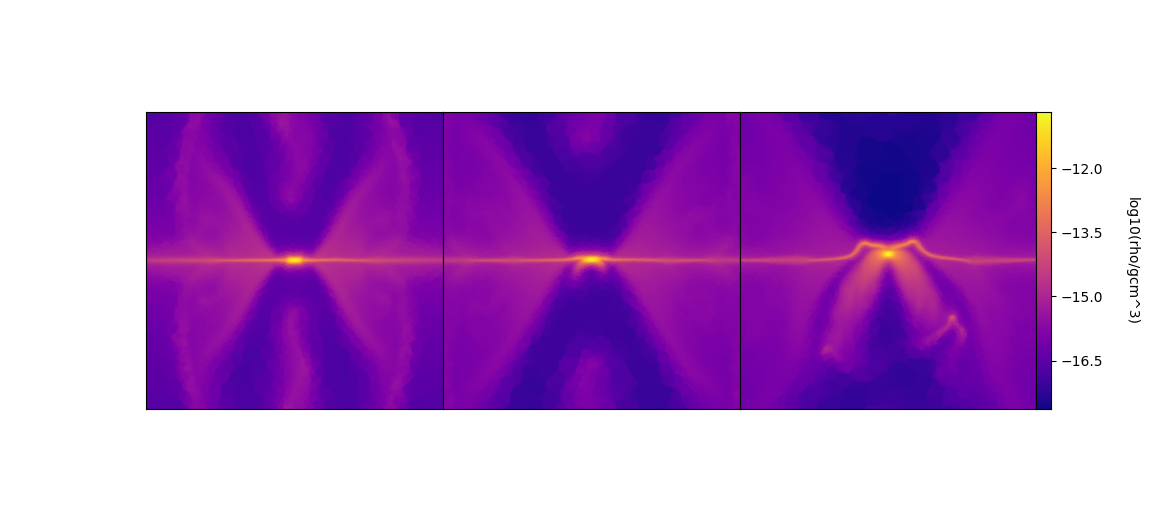
\includegraphics[width=18cm]{explosion.png}
		\caption{Result of running with a variable B field divergence cleaning speed, for the $\mu$=5, 32 cell resolution case. Panels correspond to 1.074, 1.089 and 1.103 $\tau_{ff}$.}
		\label{fig:explode}
\end{figure*}


\begin{figure*}[h!]
         \centering
		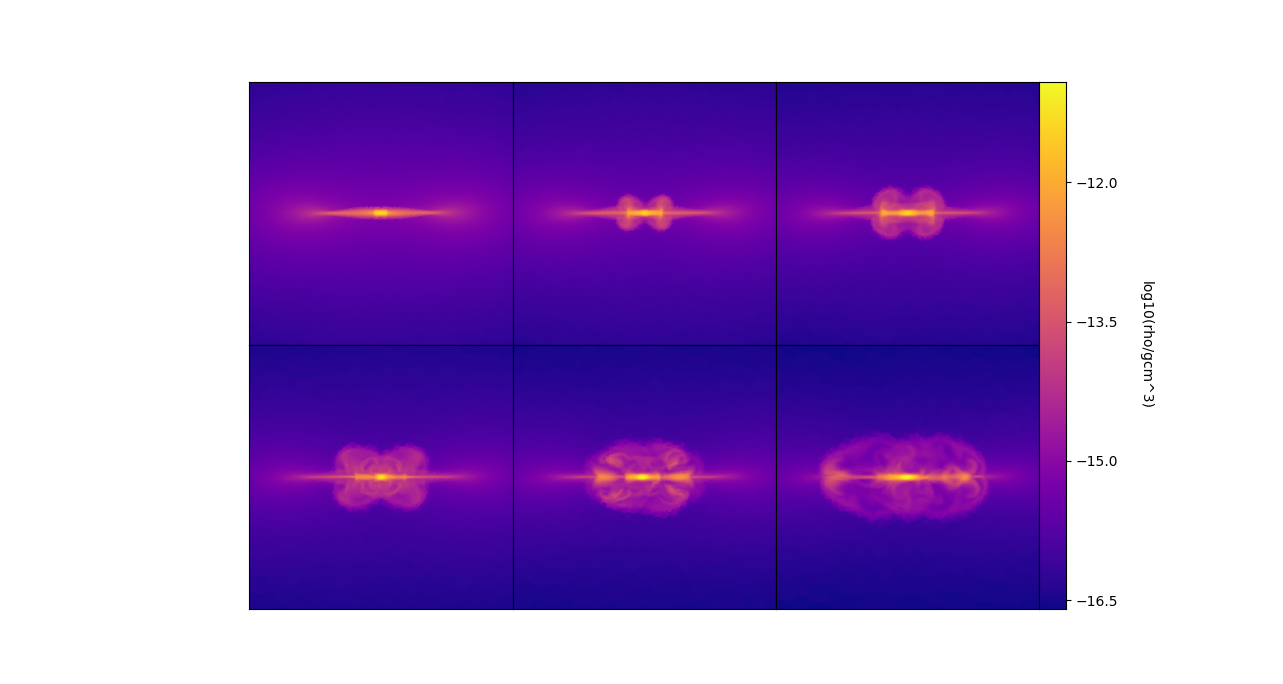
\includegraphics[width=18cm]{burzle.png}
		\caption{Top: Integrated mean density over a thin slice in the y-axis, for an initially very supercritical cloud with $\mu$=20. Images correspond to 1.030, 1.045 and 1.059 $\tau_{ff}$. Middle: Velocity magnitude shown in colour, with vector direction shown by arrows. Arrows have all been normalised to unit vectors. Bottom: Ratio of toroidal to poloidal magnetic field strength. Panels have a side length of $\sim$400AU.}
		\label{fig:burzle}
\end{figure*}




\begin{figure*}[h!]
         \centering
		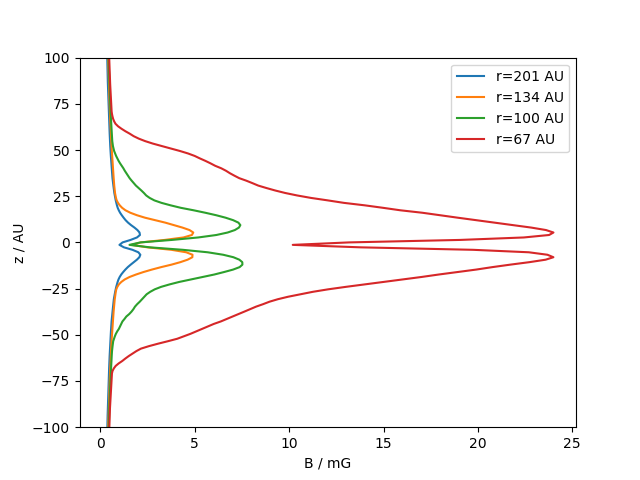
\includegraphics[width=13cm]{BvsZ_mu20.png}
		\caption{Magnetic field strength as a function of height on the axis of rotation $z$ for different radii in the xy plane, for the $\mu$=20 case.}
		\label{fig:BvsZ}
\end{figure*}


\begin{figure*}[h!]
         \centering
		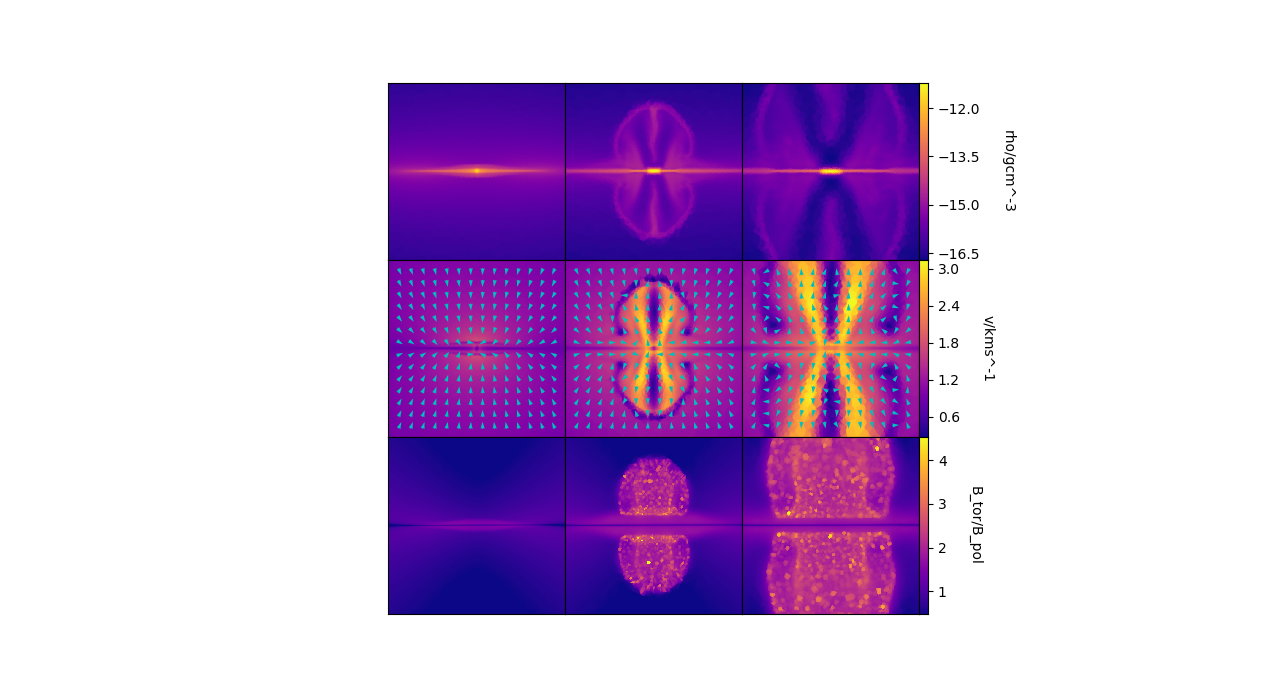
\includegraphics[width=18cm]{burzle2.png}
		\caption{Top: Integrated mean density over a thin slice in the y-axis, for an initially highly magnetised supercritical cloud with $\mu$=5. Middle: Velocity magnitude shown in colour, with vector direction shown by arrows. Bottom: Ratio of toroidal to poloidal magnetic field strengthPanels correspond to 1.030, 1.060 and 1.089 $\tau$\textsubscript{ff}. Panel size $\sim$800AU.}
		\label{fig:burzle2}
\end{figure*}





\subsection{Discussion}
\label{sub:discussion1}

Initially, the version of AREPO used contained a module to dampen divergence errors in the magnetic field as described in \cite{Dedner2002}, but with a variable cleaning time step, however this resulted in non-physical effects. \autoref{fig:explode} shows the result of running the simulation with this module enabled, the central object appears to fall out of the disc, accompanied by an outflow of material in the other direction. As this has not occurred in any other simulation papers, or in observations of present-day star formation, the module was switched off for subsequent runs. This resulted in much longer run times due to the global time step.
In the $\mu$=20, 16 cell resolution case, a  disk formed around the central object and quickly fragmented shortly after any outlofw activity, disturbing the symmetry of the systemand preventing further outflows. With 32 cell resolution, the disk remained stable during the formation of the first core. As in \cite{Hennebelle2008} and \cite{Bate2014}, symetric outflows emerged  from the outer parts of the disk (\autoref{fig:burzle}), forming a tourus structure. The outflows reached a maximum scale of $\sim$20AU with velocities $\sim$2kms\textsuperscript{-1}. High values of B\textsubscript{toridal}/B\textsubscript{poloidal} support that the outflows are caused by magneto-rotational effects described by /\cite{Blandford1982} and \cite{Lynden-Bell2003}, while  \autoref{fig:BvsZ} shows that magnetic pressure gradiants are also present.  \autoref{fig:burzle} row 2 shows that collapse occured through the axis of rotation and through the disc, but also that outflowing mass from the outer disk was brought back in through axis of rotation. The results deviate from \cite{Burzle2011} as they obtain a secondary outflow which emerges from the central disk, which could be interpreted as the jet usually seen from a second core, although they noted that a different barotropic equation of state would be needed for that stage in the collapse.
For the $\mu$=5, 32 cell resolution case, the highly magnetised supercritical cloud was still able to collapse to form a disk around the first core (\autoref{fig:burzle2}). Compared to the $\mu$=20 case,  larger, faster ($\sim$3kms\textsuperscript{-1}) outflows emerged, with a similar structure to \cite{Machida2014} and \cite{Bate2014}. These studies involve a thermal treatment suitable of following the collapse to the formation of the prestellar core, where high velocity, centralised jets  emerged. Once again, high values of B\textsubscript{toridal}/B\textsubscript{poloidal} in outflow regions suggest that magneto-rotational effects caused the outflows. 


\section{Divergence cleaning test}
\label{sub:divclean}
The outcome seen in \autoref{fig:explode} is similar to Figure 21 in \cite{Tricco2012}, where a build up of artificial divergence in the magnetic field lead to errors in angular momentum conservation. Their method of testing the divergence cleaning was to create a small 'blob' where a divergent magnetic field (fake field) exists, within a box of non-divergent (real) field. The same test was set up to test see how varying the cleaning timestep in the \cite{Dedner2002} cleaning scheme effected the evolution of the fake field. Firstly, the fake field blob was placed in a medium of constant density with uniform velocity. Secondly, the ball was placed in a static medium with with a density step to a region where the density was enhancement by a factor of 2. \autoref{fig:noshock} shows that both a global and varied cleaning timestep converge to the same maximum and average fake field values in the medium of constant density, but that varying the cleaning rate achieves the final value faster. The maximum fake field is reduced from the initial strength, but the average fake field strength increased. \autoref{fig:static} shows that in the presence of a density enhancement, cleaning is not able to bring the fake field down to strengths below its initial value, but it does prevent it from growing indefinitely if a global cleaning rate is used. In contrast to the uniform density and velocity test, the variable cleaning rate leads to a run-away growth of the fake field.

\begin{figure*}[h!]
         \centering
		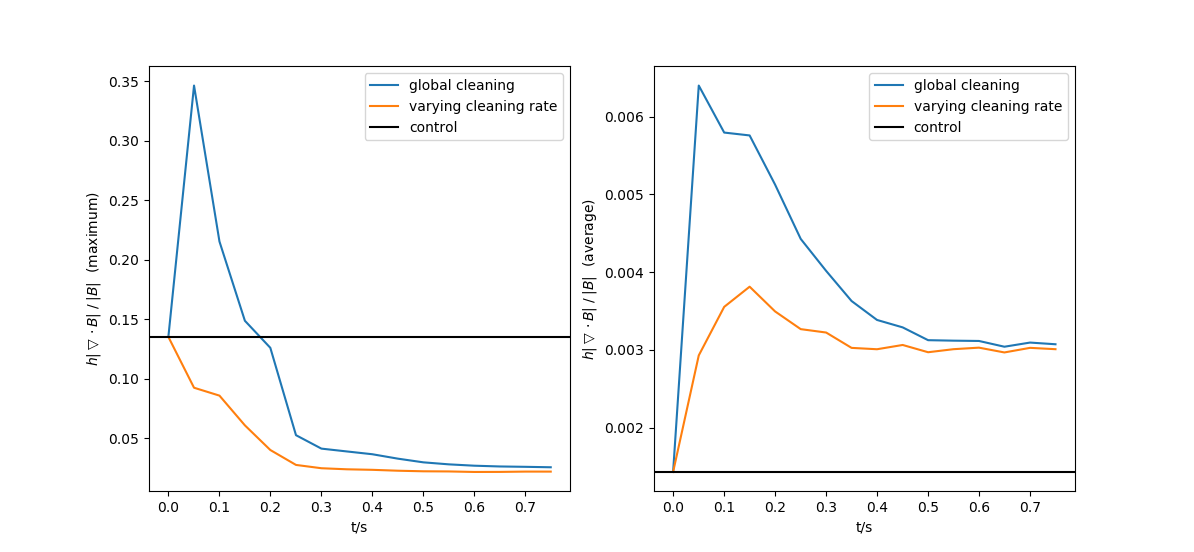
\includegraphics[width=18cm]{noshock.png}
		\caption{Performances of the \cite{Dedner2002} divergence cleaning with global and varied cleaning timesteps, for a ball of divergent fake field in a medium of constant density, with uniform velocity. The black line shows the initial values of the divergent field.}
		\label{fig:noshock}
\end{figure*}

\begin{figure*}[h!]
         \centering
		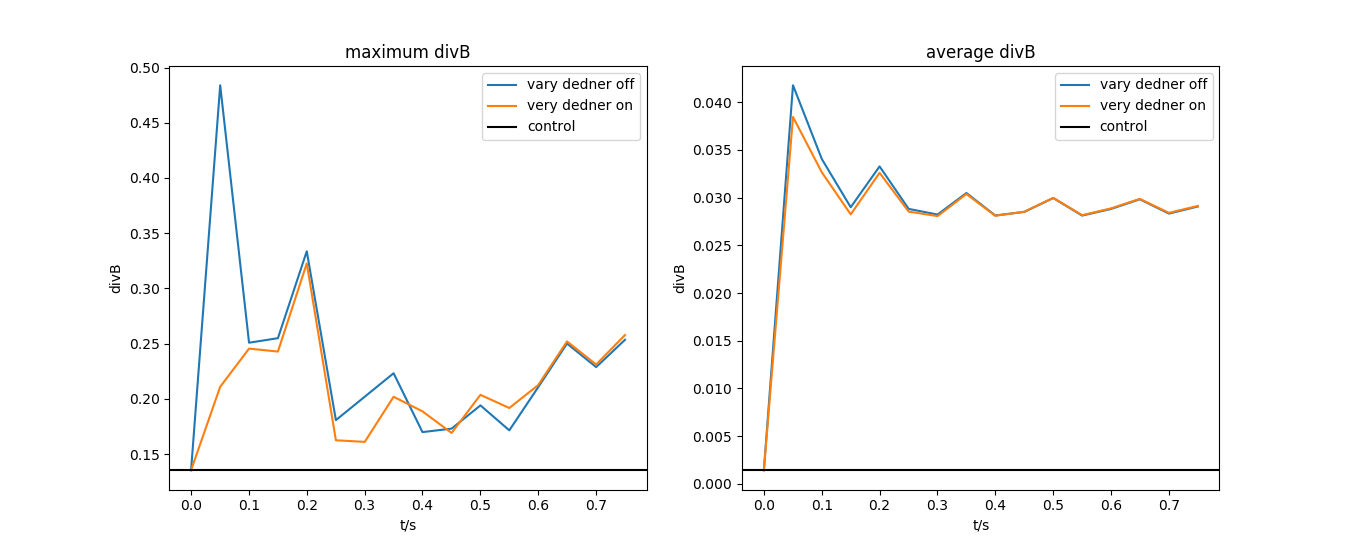
\includegraphics[width=18cm]{divB_static.png}
		\caption{Performances of the \cite{Dedner2002} divergence cleaning with global and varied cleaning timesteps, for a ball of divergent fake field in an initially static medium in the presence of a X2 density jump. The black line shows the initial values of the divergent field.}
		\label{fig:static}
\end{figure*}

\section{Population III resolution study}
\label{sub:popIIIme}
\subsection{Set-up and Initial conditions}
\label{sub:ics2}
As the environment in which Pop III star formation takes place is vastly different from its present day counterpart i.e. much higher temperatures and gas mainly composed of Hydrogen and Helium, the typical prestellar densities are less well known than in present day simulations. Hence, mulitple realisations were performed with different sink particle creation densities, to investigate the evoltion of sink masses in hopes to find a creation density above which the population of sink masses converges. The simulations were run in the absence of magnetic fields for simplicity. A cloud with a Boner Ebert density profile defined by a central density of \num{3.7e-20}gcm\textsuperscript{-3}  was placed in an ISM of density \num{2e-22}gcm\textsuperscript{-3} and temperature 200K. The cloud radius was 7.48pc, within a box of side length 7.48pc. Firstly, the cloud was allowed to evolve with no turbulence or rotation, with very low resolution ($\sim$500 cells) to create a rough relationship between density and temperature. This was done in order to model the Jeans length as a function of density, to find appropriate sink particle radii at the different formation densities. Once the sink particle radii were estimated, the gravitational softening length was chosen to be double the sink radius and the minimum cell size was chosen such that 8 cells span across the sink radius. From the low resolution run, the time evolution of maximum density per snapshot was used to select snapshot times that under sample the uneventful earlier stages of the collapse with logarithmically spaced time intervals, which switches to linearly spaced intervals in the later stages of collapse at a time chosen based on the rate of change of central density. \ref{fig:times} shows the chosen snapshot times for the subsequent higher resolution runs. Cutting down the amound of snapshots in this way saves the code having to enforce a global time step in uneventful  stages of the collapse, cutting down the run time. A turbulent velocity field was generated with a power spectrum $P(k) \propto k^{-4}$, with a ratio of turbulent to gravitational energy $\alpha_{turb}$=0.05. The sink creation density was increased by an order of magnitude for each run.

\begin{figure*}[h!]
         \centering
		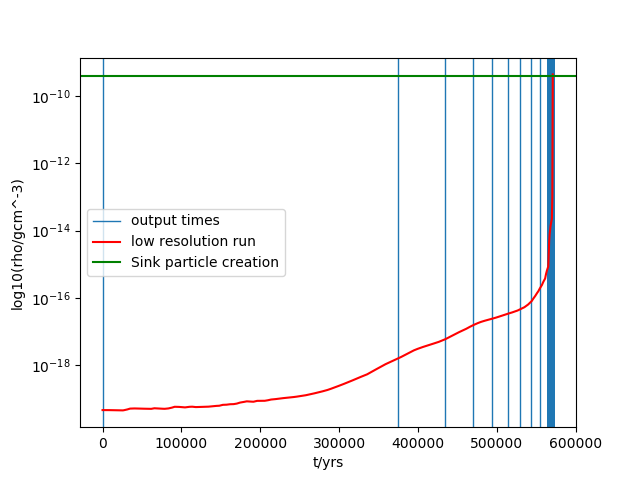
\includegraphics[width=12cm]{times_turb.png}
		\caption{}
		\label{fig:times}
\end{figure*}



\subsection{Discussion}
\label{sub:discussion2}


\bibliographystyle{apacite}
\bibliography{references}



\end{document}